\documentclass[12pt]{article}
\usepackage[margin=0.8in]{geometry}
\usepackage[utf8]{inputenc}
\usepackage{graphicx}
\usepackage[export]{adjustbox}
\usepackage{amsmath}
\usepackage{amsfonts}
\usepackage{amssymb}
\usepackage[version=4]{mhchem}
\usepackage{stmaryrd}
\usepackage{bbold}
%\usepackage[fallback]{xeCJK}
\usepackage{polyglossia}
\usepackage{fontspec}
\usepackage{censor}
%\setCJKmainfont{Noto Serif CJK TC}
\graphicspath{ {../Images/} }
\usepackage{enumitem}
\usepackage{tikz}
\usepackage{amsthm}
\usepackage{tcolorbox}
\usepackage{array}
\usepackage{tabularray}
\usepackage{makecell}
\usepackage{esvect}
%\usepackage{changepage}   % for the adjustwidth environment
\usepackage{enumitem}

\tcbuselibrary{theorems}

\definecolor{GrayCen}{HTML}{d2d2d2}
\definecolor{GrayBG}{HTML}{d9d9d9}
\definecolor{BlueDef}{HTML}{104e8b}
\definecolor{GreenProp}{HTML}{025540}
\definecolor{RedMet}{HTML}{cd5556}
\definecolor{BlackSav}{HTML}{000000}
\def\censorcolor{GrayCen}
\let\svcensorrule\censorrule
\renewcommand\censorrule[1]{%
\textcolor{\censorcolor}{\svcensorrule{#1}}}

\newtcbtheorem
[]% init options
{definition}% name
{Définition}% title
{%
  colback=GrayBG,
  colframe=BlueDef,
  fonttitle=\bfseries,
}% options
{def}% prefix

\newtcbtheorem
[]% init options
{proposition}% name
{Proposition}% title
{%
  colback=GrayBG,
  colframe=GreenProp,
  fonttitle=\bfseries,
}% options
{prop}% prefix

\newtcbtheorem
[]% init options
{method}% name
{Méthode}% title
{%
  theorem name,
  colback=GrayBG,
  colframe=RedMet,
  fonttitle=\bfseries,
}% options
{met}% prefix

\newtcbtheorem
[]% init options
{savoir}% name
{Savoir-faire du chapitre}% title
{%
  theorem name,
  colback=GrayBG,
  colframe=BlackSav,
  fonttitle=\bfseries,
}% options
{sav}% prefix

\newtheoremstyle{break}
{\topsep}{\topsep}%
{}{}%
{\bfseries}{}%
{\newline}{}%
\theoremstyle{break}
\newtheorem*{example}{Exemple.}
\newtheorem*{remark}{Remarque.}

\newenvironment{demo}[1][\proofname]{%
  \begin{proof}[#1]$ $\newline
  }{%
  \end{proof}
}

\setmainlanguage{french}
%\setmainfont{CMU Serif}

\title{
  \vspace{4em}
  \centering
  \tcbset{colframe=BlackSav,colback=GrayBG}
  \tcbox[tikznode]{
    Chapitre 8 \\Applications du produit scalaire
  }
}

\author{}
\date{}

\setlength\parindent{0pt}
%\setlist[itemize]{topsep=0pt}
\setlist{nolistsep}
%\setlist[itemize]{noitemsep}
%\setlist[enumerate]{noitemsep}

\newcolumntype{C}[1]{>{\centering\arraybackslash}m{#1}}
\newcolumntype{L}[1]{>{\raggedright\arraybackslash}m{#1}}
\newcolumntype{N}{@{}m{0pt}@{}}

\begin{document}
\maketitle

\tableofcontents

%\newcommand{\hideM}[1]{\mbox{\vphantom{$#1$}\smash{\colorbox{gray!50}{$\displaystyle #1$}}} }
%\newcommand{\hide}[1]{\mbox{\vphantom{#1}\smash{\colorbox{gray!50}{#1}}}}
\newcommand{\hideM}[1]{\mbox{\vphantom{$#1$}\smash{\colorbox{gray!50}{\phantom{$\displaystyle #1$}}}} }
\newcommand{\hide}[1]{\mbox{\vphantom{#1}\smash{\colorbox{gray!50}{\phantom{#1}}}}}

\newpage

Dans toute la suite, on se place dans un repère orthonormé $(\mathrm{O} ; \vec{i}, \vec{j})$.

\section{Application à l'étude des droites}
\begin{definition}{}{}
  Soit $D$ une droite. On appelle \hide{vecteur normal} à $D$ tout vecteur non nul qui est orthogonal à un vecteur directeur de $D$.
\end{definition}

\begin{remark}
  De la même manière qu'il existe une infinité de vecteurs directeurs d'une droite, il existe aussi une infinité de vecteurs normaux à une droite.
\end{remark}

\begin{proposition}{}{}
  Soient $D$ et $D^{\prime}$ deux droites du plan. Les conditions suivantes sont équivalentes:\\
  (i) $D$ et $D^{\prime}$ sont perpendiculaires;\\
  (ii) Il existe un vecteur directeur de $D$ et un vecteur directeur de $D^{\prime}$ qui sont \hide{orthogonaux} ;\\
  (iii) Il existe un vecteur normal à $D$ et un vecteur normal à $D^{\prime}$ qui sont \hide{orthogonaux} ;
\end{proposition}

\begin{proof}
  \begin{enumerate}
    \itemindent=-15pt
    \item[]
    \item[]\textbf{(i)} $\Longrightarrow$ \textbf{(ii)} Cela découle immédiatement de la définition de deux vecteurs orthogonaux.
    \item[]\textbf{(ii)} $\Longrightarrow$ \textbf{(iii)} Supposons qu'il existe un vecteur $\vec{u}$ directeur de $D$ et un vecteur $\vec{v}$ directeur de $D^{\prime}$ tels que $\vec{u}$ et $\vec{v}$ soient orthogonaux. D'après la définition d'un vecteur normal (Définition 1), $\vec{u}$ est un vecteur normal à $D^{\prime}$. De même, $\vec{v}$ est normal à $D$. Comme $\vec{u}$ et $\vec{v}$ sont orthogonaux, la propriété est vérifiée.
    \item[]\textbf{(iii)} $\Longrightarrow$ \textbf{(i)} Supposons qu'il existe un vecteur $\vec{u}$ normal à $D$ et un vecteur $\vec{v}$ normal à $D^{\prime}$ tels que $\vec{u}$ et $\vec{v}$ soient orthogonaux. Comme $\vec{u}$ est normal à $D$, il existe un vecteur directeur $\vec{k}$ de $D$ tel que $\vec{u}$ est orthogonal à $\vec{k}$. Ainsi, $\vec{u}$ est orthogonal à $\vec{k}$ et à $\vec{v}$. C'est donc que $\vec{k}$ et $\vec{v}$ sont colinéaires et que, par conséquent, $\vec{v}$ est un vecteur directeur de $D$. De même on montre que $\vec{u}$ est un vecteur directeur de $D^{\prime}$. Les droites $D$ et $D^{\prime}$ ont des vecteurs directeurs orthogonaux et sont donc perpendiculaires.
  \end{enumerate}
\end{proof}

\begin{proposition}{}{}
  Soient $a, b, c \in \mathbb{R}$ tels que $(a ; b) \neq(0 ; 0)$.

  \begin{itemize}
    \item La droite d'équation cartésienne $a x+b y+c=0$ admet pour vecteur normal le vecteur $\vec{n}\dbinom{\hideM{a}}{\hideM{b}}$.
    \item Réciproquement, toute droite ayant pour vecteur normal le vecteur non nul $\vec{n}\dbinom{a}{b}$ admet une équation cartésienne de la forme $a x+b y+c=0$.
  \end{itemize}
\end{proposition}

\begin{demo}
  Il suffit de se rappeler qu'un vecteur directeur de la droite d'équation $a x+b y+c=0$ est le vecteur $\vec{u}\dbinom{-b}{a}$. Ainsi, $\vec{u} \cdot \vec{n}=(-b) \times a+a \times b=0$, et donc $\vec{u}$ et $\vec{n}$ sont orthogonaux.
\end{demo}

\begin{example}
  Soit $D$ la droite d'équation $2 x+3 y+5=0$ et $D^{\prime}$ la droite d'équation $6 x-4 y+1=0$. Montrer que les deux droites $D$ et $D^{\prime}$ sont perpendiculaires.

  ~\\Solution :\\
  $\vec{n}\dbinom{2}{3}$ est un vecteur normal à $D$ et $\vec{m}\dbinom{6}{-4}$ est un vecteur normal à $D^{\prime}$.\\
  D'après la Proposition 1, il suffit de montrer que $\vec{n}$ et $\vec{m}$ sont orthogonaux. Or,

  $$
  \vec{n} \cdot \vec{m}=2 \times 6+3 \times(-4)=0 .
  $$
\end{example}

\section{Application à l'étude des cercles}
\begin{definition}{}{}
  On appelle cercle de centre $\Omega$ et de rayon $r$, noté $\hideM{\mathcal{C}_{(\Omega, r)}}$ l'ensemble des points M du plan tels que $\Omega \mathrm{M}=r$.
\end{definition}

\begin{proposition}{}{}
  Soient $a, b \in \mathbb{R}$. Une équation du cercle de centre $\Omega(a ; b)$ et de rayon $r$ est :

  $$
  \mathrm{M}(x ; y) \in \mathcal{C}_{(\Omega, r)} \Longleftrightarrow(x-a)^{2}+(y-b)^{2}=\hideM{r^{2}}
  $$
\end{proposition}

\begin{demo}

  $$
  \begin{aligned}
    M \in \mathcal{C}_{(\Omega, r)} & \Longleftrightarrow \Omega M=r \\
    & \Longleftrightarrow \sqrt{(x-a)^{2}+(y-b)^{2}}=r \quad(\text { car le repère est orthonormé }) \\
    & \Longleftrightarrow(x-a)^{2}+(y-b)^{2}=r^{2} \text { car } r>0
  \end{aligned}
  $$
\end{demo}

\begin{method}{Déterminer le centre et le rayon d'un cercle défini par une équation}{}
  \begin{itemize}
    \item Mettre l'équation sous la forme $x^{2}+a x+y^{2}+b y+c=0$
    \item Commencer à factoriser sous la forme $\left(x-\frac{a}{2}\right)^{2}+\left(y-\frac{b}{2}\right)^{2}+\ldots=0$
    \item Simplifier les constantes.
  \end{itemize}
\end{method}

\begin{example}
  On considère le cercle $\mathcal{C}$ d'équation $x^{2}+y^{2}-2 x=-3 y-2$.\\
  Déterminer le centre et le rayon de $\mathcal{C}$.

  \newpage
  Solution :

  $$
  \begin{aligned}
    \mathrm{M}(x ; y) \in \mathcal{C} & \Longleftrightarrow x^{2}+y^{2}-2 x=-3 y-2 \\
    & \Longleftrightarrow x^{2}-2 x+y^{2}+3 y+2=0 \\
    & \Longleftrightarrow(x-1)^{2}+\left(y+\frac{3}{2}\right)^{2}+2-1-\frac{9}{4}=0 \\
    & \Longleftrightarrow(x-1)^{2}+\left(y+\frac{3}{2}\right)^{2}-\frac{5}{4}=0 \\
    & \Longleftrightarrow(x-1)^{2}+\left(y+\frac{3}{2}\right)^{2}=\left(\frac{\sqrt{5}}{2}\right)^{2}
  \end{aligned}
  $$

  Ainsi, $\mathcal{C}$ est le cercle de centre $\Omega\left(1 ;-\frac{3}{2}\right)$ et de rayon $\frac{\sqrt{5}}{2}$.
\end{example}

\begin{proposition}{}{}
  Soient A et B deux points distincts du plan. L'ensemble des points M du plan tels que $\hideM{\overrightarrow{\mathrm{MA}} \cdot \overrightarrow{\mathrm{MB}}=0}$ est le cercle de diamètre $[\mathrm{AB}]$.
\end{proposition}

\begin{demo}
  Soit $\mathrm{M}(x ; y)$ les coordonnées de M dans un repère orthonormé.

  $$
  \begin{aligned}
    \overrightarrow{\mathrm{MA}} \cdot \overrightarrow{\mathrm{MB}}=0 & \Longleftrightarrow\left(x-x_{A}\right)\left(x-x_{B}\right)+\left(y-y_{A}\right)\left(y-y_{B}\right)=0 \\
    & \Longleftrightarrow x^{2}-x_{A} x-x_{B} x+x_{A} x_{B}+y^{2}-y_{A} y-y_{B} y+y_{A} y_{B}=0 \\
    & \Longleftrightarrow x^{2}-\left(x_{A}+x_{B}\right) x+y^{2}-\left(y_{A}+y_{B}\right) y+x_{A} x_{B}+y_{A} y_{B}=0 \\
    & \Longleftrightarrow\left(x-\frac{x_{A}+x_{B}}{2}\right)^{2}+\left(y-\frac{y_{A}+y_{B}}{2}\right)^{2}-\left(\frac{x_{A}+x_{B}}{2}\right)^{2}-\left(\frac{y_{A}+y_{B}}{2}\right)^{2}+x_{A} x_{B}+y_{A} y_{B} \\
    & \Longleftrightarrow\left(x-\frac{x_{A}+x_{B}}{2}\right)^{2}+\left(y-\frac{y_{A}+y_{B}}{2}\right)^{2}=\frac{\left(x_{A}-x_{B}\right)^{2}+\left(y_{A}-y_{B}\right)^{2}}{4} \\
    & \Longleftrightarrow\left(x-\frac{x_{A}+x_{B}}{2}\right)^{2}+\left(y-\frac{y_{A}+y_{B}}{2}\right)^{2}=\left(\frac{\mathrm{AB}}{2}\right)^{2}
  \end{aligned}
  $$

  ce qui est bien une équation du cercle de diamètre $[\mathrm{AB}]$.
\end{demo}

\newpage

\begin{proposition}{}{}
  Soient $A$ et $B$ deux points distincts du plan et soit $\mathcal{C}$ un cercle de diamètre $[\mathrm{AB}]$. On a alors l'équivalence suivante :

  $$
  \mathrm{M} \in \mathcal{C} \Longleftrightarrow \hideM{\text { AMB est rectangle en } \mathrm{M}}
  $$
\end{proposition}

\begin{center}
  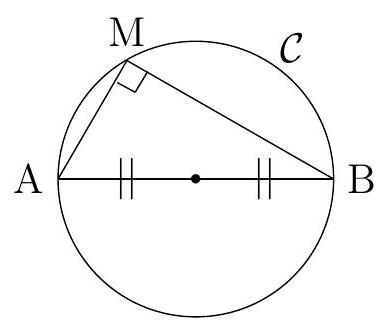
\includegraphics[width=0.25\textwidth]{2025_03_24_dc0c3465a8287f1a9b81g-4}
\end{center}

\begin{demo}
  D'après la Proposition 4,

  $$
  \begin{aligned}
    \mathrm{M} \in \mathcal{C} & \Longleftrightarrow \overrightarrow{\mathrm{MA}} \cdot \overrightarrow{\mathrm{MB}}=0 \\
    & \Longleftrightarrow(\mathrm{MA}) \perp(\mathrm{MB}) \\
    & \Longleftrightarrow \text { AMB est rectangle en } \mathrm{M}
  \end{aligned}
  $$
\end{demo}

\section{Application à l'étude des triangles}
Dans toute cette partie, on utilisera les notations suivantes:\\
$\mathrm{AB}=c, \mathrm{AC}=b, \mathrm{BC}=a, \widehat{\mathrm{BAC}}=\widehat{\mathrm{A}}, \widehat{\mathrm{ABC}}=\widehat{\mathrm{B}}$ et $\widehat{\mathrm{ACB}}=\widehat{\mathrm{B}}$.\\
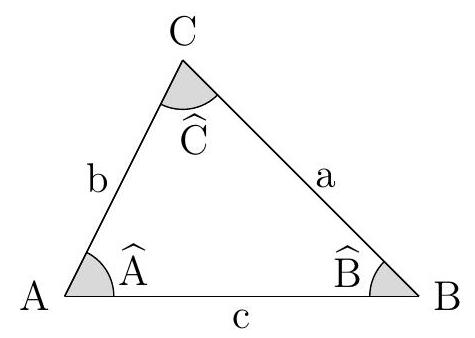
\includegraphics[width=0.3\textwidth, center]{2025_03_24_dc0c3465a8287f1a9b81g-5}

\subsection{Formule d'Al-Kashi ou théorème de Pythagore généralisé}
\begin{proposition}{}{}
  Pour tout triangle ABC,

  $$
  a^{2}=\hideM{b^{2}+c^{2}-2 b c \cos (\widehat{\mathrm{~A}})}
  $$
\end{proposition}

\begin{demo}
  $$
  \begin{aligned}
    a^{2}=\mathrm{BC}^{2}=\|\overrightarrow{\mathrm{BC}}\|^{2} & =\|(\overrightarrow{\mathrm{BA}}+\overrightarrow{\mathrm{AC}})\|^{2} \\
    & =\|\overrightarrow{\mathrm{BA}}\|^{2}+2 \overrightarrow{\mathrm{BA}} \cdot \overrightarrow{\mathrm{AC}}+\|\overrightarrow{\mathrm{AC}}\|^{2} \\
    & =\|\overrightarrow{\mathrm{BA}}\|^{2}+\|\overrightarrow{\mathrm{AC}}\|^{2}-2 \overrightarrow{\mathrm{AB}} \cdot \overrightarrow{\mathrm{AC}} \\
    & =b^{2}+c^{2}-2 b c \cos (\overrightarrow{\mathrm{~A}})
  \end{aligned}
  $$

  (en utilisant la formule trigonométrique du produit scalaire).
\end{demo}

\subsection{La loi des sinus}
\begin{proposition}{}{}
  Pour tout triangle ABC,

  $$
  \frac{a}{\sin (\widehat{\mathrm{~A}})}=\hideM{\frac{b}{\sin (\widehat{\mathrm{~B}})}}=\hideM{\frac{c}{\sin (\widehat{\mathrm{C}})}}
  $$
\end{proposition}

\begin{demo}
  On décompose la preuve en deux étapes.

  \begin{itemize}
    \item Étape 1 : on prouve que si $\mathcal{S}$ est l'aire du triangle ABC , alors $\mathcal{S}=\frac{1}{2} b c \sin (\widehat{\mathrm{~A}})$.

      En fait, on sait que si H est le projeté orthogonal de C sur $[\mathrm{AB}]$, alors $\mathcal{S}=\frac{1}{2} \mathrm{AB} \times \mathrm{HC}$. Or, si $\widehat{\mathrm{A}}$ est un angle aigu, $\mathrm{HC}=\mathrm{AC} \sin (\widehat{\mathrm{A}})$\\
      et si $\widehat{\mathrm{A}}$ est un angle obtus, $\mathrm{HC}=\mathrm{AC} \sin (\pi-\widehat{\mathrm{A}})=\mathrm{AC} \sin (\widehat{\mathrm{A}})$ (voir les figures ci-dessous).\\
      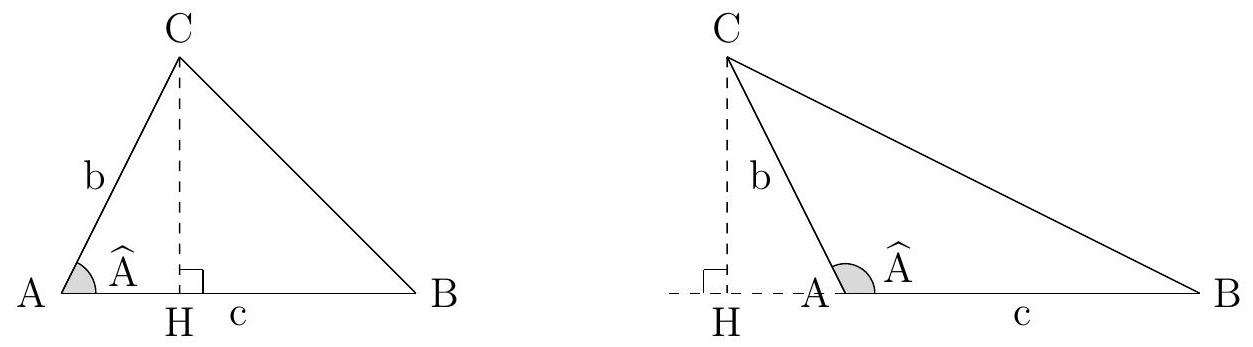
\includegraphics[width=0.8\textwidth, center]{2025_03_24_dc0c3465a8287f1a9b81g-6(1)}

      Ainsi, dans tous les cas, $\mathcal{S}=\frac{1}{2} \mathrm{AB} \times \mathrm{AC} \sin (\widehat{A})=\frac{1}{2} b c \sin (\widehat{\mathrm{~A}})$.

    \item Étape 2 : On en déduit la loi des sinus.

      D'après l'étape 1 , on peut écrire que $\mathcal{S}=\frac{1}{2} b c \sin (\widehat{\mathrm{~A}})$ mais aussi, par une démonstration similaire, que $\mathcal{S}=\frac{1}{2} a c \sin (\widehat{\mathrm{~B}})$ et que $\mathcal{S}=\frac{1}{2} a b \sin (\widehat{\mathrm{C}})$. Ainsi, ces trois formules permettent d'écrire que

      $$
      \frac{a b c}{2 \mathcal{S}}=\frac{a}{\sin (\widehat{\mathrm{~A}})}=\frac{b}{\sin (\widehat{\mathrm{~B}})}=\frac{c}{\sin (\widehat{\mathrm{C}})}
      $$
  \end{itemize}
\end{demo}

\subsection{Médianes et centre de gravité}
\begin{definition}{}{}
  Dans un triangle, la médiane issue d'un sommet est la droite qui passe par ce sommet et par le milieu du côté opposé.
\end{definition}

\begin{proposition}{(Théorème de la médiane)}
  Pour tout triangle ABC , si I est le milieu de [BC] alors :

  $$
  \mathrm{AB}^{2}+\mathrm{AC}^{2}=\hideM{2 \mathrm{AI}^{2}+\frac{\mathrm{BC}^{2}}{2}}
  $$

\end{proposition}

\begin{center}
  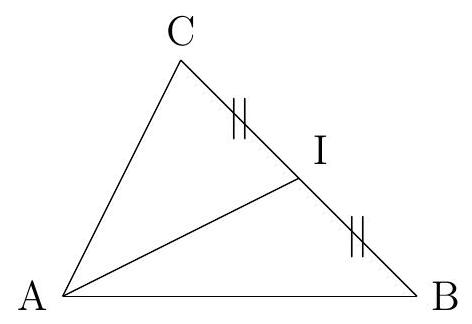
\includegraphics[width=0.3\textwidth]{2025_03_24_dc0c3465a8287f1a9b81g-6}
\end{center}

\begin{demo}
  Pour le démontrer, on fait apparaître le point I en utilisant la relation de Chasles. Plus précisément:

  $$
  \begin{aligned}
    \mathrm{AB}^{2}+\mathrm{AC}^{2} & =\overrightarrow{\mathrm{AB}}^{2}+\overrightarrow{\mathrm{AC}}^{2} \\
    & =(\overrightarrow{\mathrm{AI}}+\overrightarrow{\mathrm{IB}})^{2}+(\overrightarrow{\mathrm{AI}}+\overrightarrow{\mathrm{IC}})^{2} \\
    & =\overrightarrow{\mathrm{AI}}^{2}+2 \overrightarrow{\mathrm{AI}} \cdot \overrightarrow{\mathrm{IB}}+\overrightarrow{\mathrm{IB}}^{2}+\overrightarrow{\mathrm{AI}}^{2}+2 \overrightarrow{\mathrm{AI}} \cdot \overrightarrow{\mathrm{IC}}+\overrightarrow{\mathrm{IC}}^{2} \\
  & \left.=2 \overrightarrow{\mathrm{AI}}^{2}+2 \overrightarrow{\mathrm{AI}} \cdot \overrightarrow{\mathrm{IB}}+\overrightarrow{\mathrm{IC}}\right)+\overrightarrow{\mathrm{IB}}^{2}+\overrightarrow{\mathrm{IC}}^{2} \\
  & =2 \overrightarrow{\mathrm{AI}}^{2}+\overrightarrow{\mathrm{IB}}^{2}+\overrightarrow{\mathrm{IC}}^{2} \quad(\operatorname{car} \overrightarrow{\mathrm{IB}}+\overrightarrow{\mathrm{IC}}=\overrightarrow{0}) \\
  & =2 \mathrm{AI}^{2}+2 \mathrm{IB}^{2} \quad(\operatorname{car} \mathrm{IB}=\mathrm{IC}) \\
  & =2 \mathrm{AI}^{2}+\frac{\mathrm{BC}^{2}}{2} \quad\left(\operatorname{car} \mathrm{IB}=\frac{\mathrm{BC}}{2}\right)
\end{aligned}
$$
\end{demo}

\begin{remark}
En utilisant la même méthode et en faisant apparaître le point I à l'aide de la relation de Chasles, on peut également montrer que

$$
\overrightarrow{\mathrm{AB}} \cdot \overrightarrow{\mathrm{AC}}=\mathrm{AI}^{2}-\frac{\mathrm{BC}^{2}}{4} \text { et que } \mathrm{AB}^{2}-\mathrm{AC}^{2}=2 \overrightarrow{\mathrm{AI}} \cdot \overrightarrow{\mathrm{CB}}
$$
\end{remark}

\newpage

\begin{proposition}{}{}
Pour tout triangle $\mathrm{ABC}$, il existe un unique point $G$ tel que $\hideM{\overrightarrow{\mathrm{GA}}+\overrightarrow{\mathrm{GB}}+\overrightarrow{\mathrm{GC}}=\overrightarrow{0}}$. Ce point est appelé \textbf{centre de gravité} du triangle.
\end{proposition}

\begin{demo}
Soient A, B et C trois points du plan.

$$
\begin{aligned}
  \overrightarrow{\mathrm{GA}}+\overrightarrow{\mathrm{GB}}+\overrightarrow{\mathrm{GC}}=\overrightarrow{0} & \Longleftrightarrow \overrightarrow{\mathrm{GA}}+\overrightarrow{\mathrm{GA}}+\overrightarrow{\mathrm{AB}}+\overrightarrow{\mathrm{GA}}+\overrightarrow{\mathrm{AC}}=\overrightarrow{0} \\
  & \Longleftrightarrow 3 \overrightarrow{\mathrm{GA}}+\overrightarrow{\mathrm{AB}}+\overrightarrow{\mathrm{AC}}=\overrightarrow{0} \\
  & \Longleftrightarrow-3 \overrightarrow{\mathrm{GA}}=\overrightarrow{\mathrm{AB}}+\overrightarrow{\mathrm{AC}} \\
  & \Longleftrightarrow 3 \overrightarrow{\mathrm{AG}}=\overrightarrow{\mathrm{AB}}+\overrightarrow{\mathrm{AC}} \\
  & \Longleftrightarrow \overrightarrow{\mathrm{AG}}=\frac{1}{3} \overrightarrow{\mathrm{AB}}+\frac{1}{3} \overrightarrow{\mathrm{AC}} \\
  & \Longleftrightarrow \text { G est l'image de A par la translation de vecteur } \frac{1}{3} \overrightarrow{\mathrm{AB}}+\frac{1}{3} \overrightarrow{\mathrm{AC}} .
\end{aligned}
$$

Cela prouve donc que $G$ existe et est unique.
\end{demo}

\begin{proposition}{}{}
\begin{itemize}
  \item Les médianes d'un triangle sont concourantes (elles se coupent en un même point).
  \item Leur point d'intersection est le centre de gravité du triangle.
  \item Le centre de gravité est situé au deux tiers d'une médiane en partant du sommet dont elle est issue.
\end{itemize}
\end{proposition}

\begin{demo}
On va démontrer les trois points en même temps grâce à un calcul vectoriel.\\[0pt]
On note I le milieu de [BC], J le milieu de [AC] et K le milieu de AB.\\
Comme G est le centre de gravité de ABC , on sait, d'après la preuve de la Proposition 9, que $\overrightarrow{\mathrm{AG}}=\frac{1}{3} \overrightarrow{\mathrm{AB}}+\frac{1}{3} \overrightarrow{\mathrm{AC}}$. Ainsi, en utilisant la relation de Chasles :

$$
\begin{aligned}
  \overrightarrow{\mathrm{AG}} & =\frac{1}{3}(\overrightarrow{\mathrm{AI}}+\overrightarrow{\mathrm{IB}})+\frac{1}{3}(\overrightarrow{\mathrm{AI}}+\overrightarrow{\mathrm{IC}}) \\
  & =\frac{2}{3} \overrightarrow{\mathrm{AI}}+\frac{1}{3}(\overrightarrow{\mathrm{IB}}+\overrightarrow{\mathrm{IC}}) \\
  & =\frac{2}{3} \overrightarrow{\mathrm{AI}} \quad(\operatorname{car} \overrightarrow{\mathrm{IB}}+\overrightarrow{\mathrm{IC}}=\overrightarrow{0})
\end{aligned}
$$

De la même manière, on montre que $\overrightarrow{\mathrm{BG}}=\frac{2}{3} \overrightarrow{\mathrm{BJ}}$ et que $\overrightarrow{\mathrm{CG}}=\frac{2}{3} \overrightarrow{\mathrm{CJ}}$ Finalement, du fait de la colinéarité des vecteurs, on voit que G appartient aux trois médianes. C'est donc qu'elles sont concourantes en le point $G$. Par ailleurs, on a montré que $\mathrm{AG}=\frac{2}{3} \mathrm{AI}$, que $\mathrm{BG}=\frac{2}{3} \mathrm{BJ}$ et que $\mathrm{CG}=\frac{2}{3} \mathrm{CK}$
\end{demo}

\begin{method}[title=Différentes formules dans le triangle]{}{}
\begin{center}
  \renewcommand{\arraystretch}{1.5}
  \begin{tabular}{|c|c|c|}
    \hline
    Nom & Formule & Lien entre: \\
    \hline
    \begin{tabular}{c}
      Formule \\
      d'Al-Kashi \\
    \end{tabular} & $a^{2}=b^{2}+c^{2}-2 b c \cos (\widehat{\mathrm{~A}})$ &
    \begin{tabular}{c}
      Un angle et les longueurs \\
      des trois côtés \\
    \end{tabular} \\
    \hline
    Loi des sinus & $\dfrac{a}{\sin (\widehat{\mathrm{~A}})}=\dfrac{b}{\sin (\widehat{\mathrm{~B}})}=\dfrac{c}{\sin (\widehat{\mathrm{C}})}$ & Deux angles et leurs côtés opposés \\
    \hline
    \begin{tabular}{c}
      Théorème de \\
      la médiane \\
    \end{tabular} & $\mathrm{AB}^{2}+\mathrm{AC}^{2}=2 \mathrm{AI}^{2}+\frac{\mathrm{BC}^{2}}{2}$ &
    \begin{tabular}{c}
      La longueur d'une médiane \\
      et les longueurs des trois côtés \\
    \end{tabular} \\
    \hline
  \end{tabular}
\end{center}
\end{method}

\vfill

\begin{savoir}{}{}
\begin{itemize}
  \item Déterminer une équation cartésienne d'une droite connaissant un point et un vecteur normal.
  \item Déterminer les coordonnées du projeté orthogonal d'un point sur une droite.
  \item Reconnaître une équation de cercle, déterminer le centre et le rayon.
  \item Savoir déterminer l'ensemble des mesures (angles et longueurs) d'un triangle à partir de trois mesures données.
  \item Utiliser le produit scalaire pour résoudre un problème de géométrie.
\end{itemize}
\end{savoir}

\vfill

\end{document}